\section{Velocity Model of the Vehicle}
In this section the block named \textit{Vehicle} in \chapref{cha:ModelOfVehicle} \figref{fig:StartTotalModelsystem} is described and modelled in respect to velocity being the output of the system. In \figref{fig:Velocitymodelplantopen} the expanding of the block named \textit{Vehicle} is illustrated.

\begin{figure}[H]
	\centering
	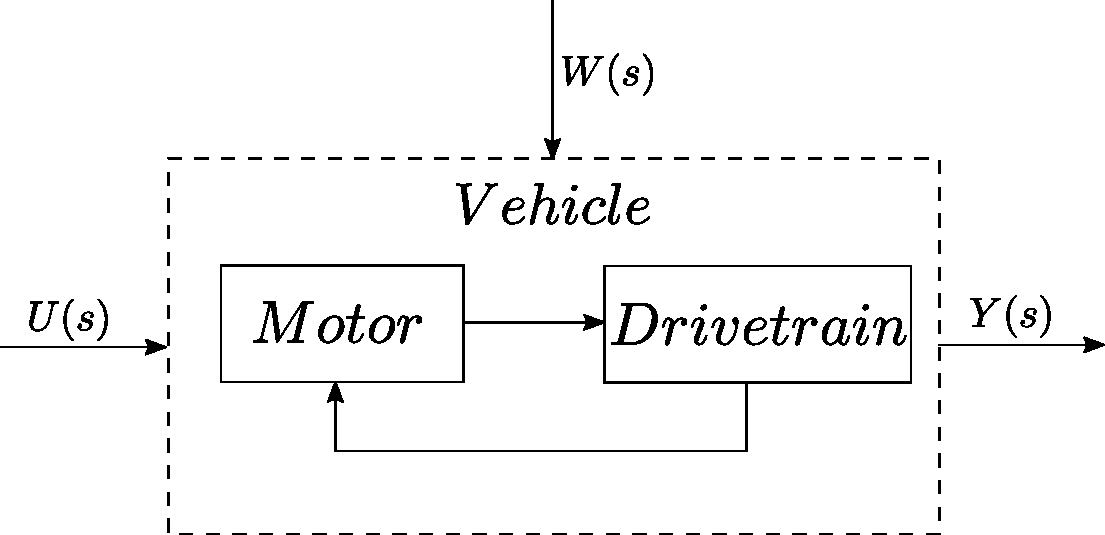
\includegraphics[scale=0.6]{figures/plantopen.pdf}
	\caption{Expanded \textit{Vehicle} block in \chapref{cha:ModelOfVehicle} \figref{fig:StartTotalModelsystem}. The figure only illustrates the velocity of the vehicle when it is driving in a straight line.}
	\label{fig:Velocitymodelplantopen}
\end{figure}

\todo{When making the overall system get this streamlinned, Rasmus comment, there must be other things. Futhermore describe what is in the figure.}

The velocity model of the vehicle has been split up into a motor and a drivetrain section. The motor receives an input from the controller, $U(s)$, regulating its supplied voltage. In return, the motor delivers a rotational force, $\tau(s)$ as an output to the drivetrain. The drivetrain generates the actual linear velocity as the output of the \textit{Vehicle} block, $Y(s)$. Furthermore is the drivetrain supplying the motor with an angular velocity, $\omega_m(s)$. The angular velocity  is dependent on the total inertia of the system, and will thereby ensure that the motor is affected by its load. The two sections, the motor and the drivetrain, is derived by only considering the parameters affecting the vehicle, when the vehicle is driving in a straight line. Thus, excluding the differential steering, see \todo{reference to differential steering}, and thereby only modelling the system when the wheels have exactly the same velocity.

In the following subsection the motor section in \figref{fig:Velocitymodelplantopen} will be modelled.